\documentclass[11pt]{scrartcl}

\title{Anforderungsspezifikation}
\author{Silvan Adrian \\ Fabian Binna}
\date{\today{}}

\usepackage[ngerman]{babel}
\usepackage[automark]{scrpage2}
\usepackage[colorlinks = true,
linkcolor = black]{hyperref}
\usepackage{color}
\usepackage[normalem]{ulem}
\usepackage{scrpage2}
\usepackage{graphicx}
\usepackage{tabularx}
\usepackage{longtable, tabu}
\graphicspath{ {../22_Grafiken/01_Logo/}{images/}{../../22_Grafiken/01_Logo/} }
\pagestyle{scrheadings}

\clearscrheadfoot
\ihead{
\includegraphics[scale=0.3]{SDDC}}
\ohead{Projekt: SDDC}
\ifoot{Template}
\cfoot{Version: 1.00}
\ofoot{Datum: \today{}}
\setheadsepline{0.5pt}
\setfootsepline{0.5pt}

\usepackage{ucs}
\usepackage[utf8]{inputenc}
\usepackage[T1]{fontenc}


\begin{document}
\def\arraystretch{1.5}
\begin{titlepage}
\begin{center}
\vspace{10em}

\includegraphics[scale=2]{SDDC}
\vspace{10em}
\end{center}
\begin{center}
\huge {Anforderungsspezifikation}
\end{center}
\begin{center}
\vspace{10em}
\LARGE {Silvan Adrian} \\
\LARGE {Fabian Binna}
\end{center}

\end{titlepage}

\newpage
\section{Änderungshistorie}
\begin{tabularx}{\linewidth}{l l X l}
\textbf{Datum} & \textbf{Version} & \textbf{Änderung}  & \textbf{Autor} \\
\hline
\textbf{02.10.15} & 1.00 & Erstellung des Dokuments & Gruppe \\
\textbf{02.10.15} & 1.01 & Nicht funktionale Anforderungen & Silvan Adrian\\
\textbf{02.10.15} & 1.02 & Use Cases Aktoren + User Stories Aktoren & Silvan 
Adrian\\

\end{tabularx}

\newpage
\tableofcontents
\newpage

\section{Einführung}
\subsection{Zweck}
Dieses Dokument beinhaltet die Anforderung zur Analyse.
\subsection{Gültigkeitsbereich}
Dieses Dokument ist während des ganzen Projekts gültig.


\subsection{Referenzen}
-

\section{Anforderungen}
\subsection{API}


\subsection{Customer-Dashboard}
\subsubsection{Homescreen}
Im Homescreen (sobald der Customer auf das Dashboard zugreift) werden alle zu 
Verfügung stehenden Services angezeigt.
Hier werden die Services Offerings genannt um eine Unterscheidung zwischen 
Abonnierten Services (Services) und zur Verfügung stehenden Services (Offerings) 
machen zu können.

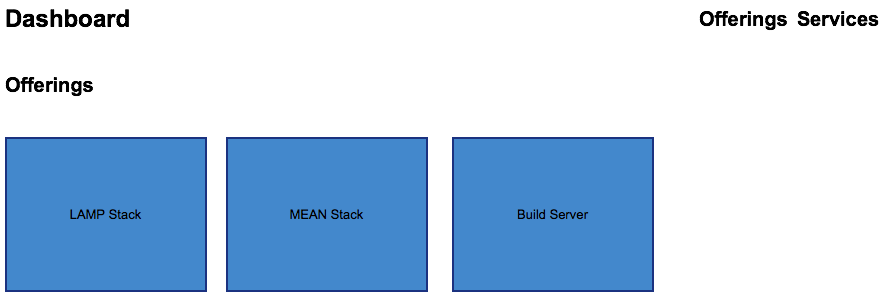
\includegraphics[width=\textwidth]{homescreen_customer}

\subsubsection{Services Übersicht}
In der Services Übersicht werden dem Customer alle abonnierten Services 
angezeigt und können hier auch gekündigt werden.

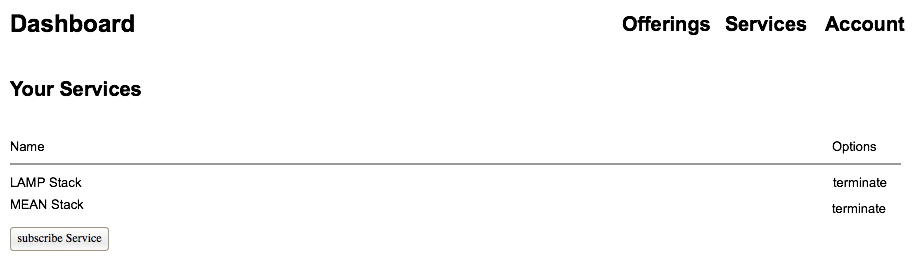
\includegraphics[width=\textwidth]{services_overview}


\subsubsection{Service abonnieren}
Sobald ein Service auf dem Homescreen ausgewählt wird muss noch der zuständige 
Provider gewählt werden (häng auch wieder davon ab von welchem Provider bisher Logindaten hinterlegt 
wurden).
Da momentan noch kein Hybrid Betrieb vorgesehen ist muss ein Account gewählt 
werden unter welchem der Service verrechnet wird.

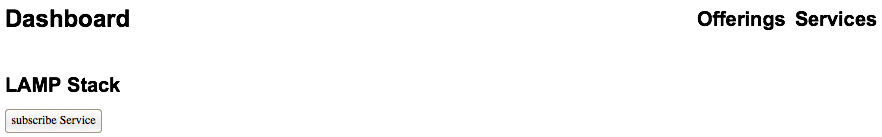
\includegraphics[width=\textwidth]{service_settings}

\subsubsection{Cloud Credentials}
Da für jeden Provider wieder Logindaten benötigt werden müssen diese an einer 
zentralen Stelle gespeichert werden (anhand von denen kann sich auch das Service Angebot 
ändern).

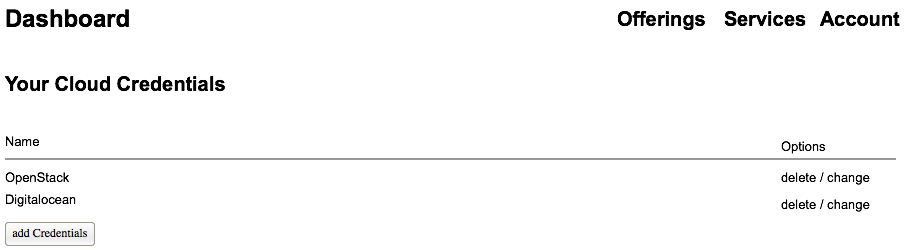
\includegraphics[width=\textwidth]{service_accounts}

\subsection{Admin-Dashboard}
Zusätzlich zum Customer-Dashboard soll ein Admin-Dashboard zur Verfügung stellen 
in welchem der Admin Services und Servicemodule erstellen kann.

\subsubsection{Service}
Ein Service hat einen bestimmten Namen und jedem Service sind eine gewisse 
Anzahl Servicemodule zugeteilt. um den Service abbilden zu können.
Hier kann der Admin den Service ändern und je nach Anforderung den Service 
anpassen.

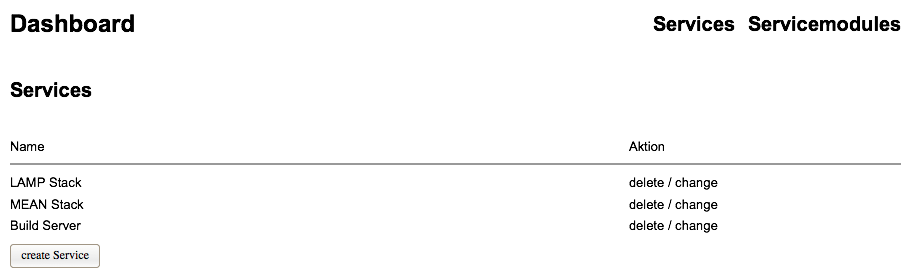
\includegraphics[width=\textwidth]{homescreen_admin}

\subsubsection{Servicemodul}
Jedes Servicemodul besitzt einen Namen und wird einem Provider zugeschrieben, 
dabei kann jedes Servicemodule den Typ Compute,Network oder Storage haben.

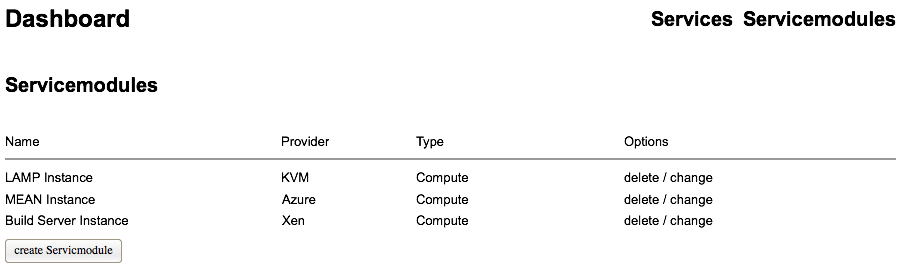
\includegraphics[width=\textwidth]{servicemodules_admin}

\section{Use Cases}
\subsection{Use Case Diagramm}
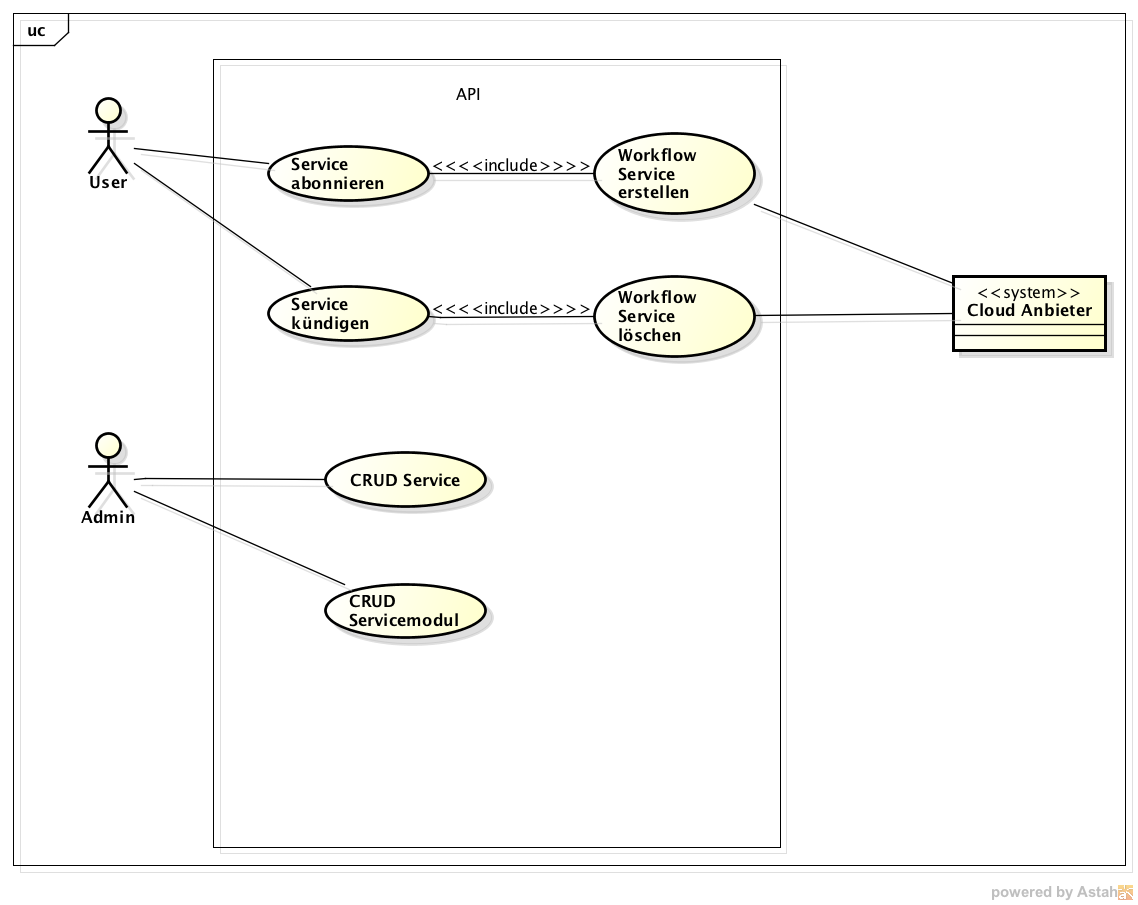
\includegraphics[width=\textwidth]{UseCase-Diagramm}
\subsection{Aktoren \& Stakeholders}
\subsubsection{Customer}
Als Customer möchte ich meine abonnierten Services verwalten.
\\
\begin{tabularx}{\linewidth}{l l X }
  \textbf{Aktor} & \textbf{Typ} & \textbf{Ziele}\\
  \hline
  Customer & Primary & 
  \begin{minipage}{5in}
  \vskip 4pt
  \begin{itemize}
    \item Service abonnieren
    \item Service kündigen
  \end{itemize}
  \vskip 4pt
 \end{minipage}\\
 \hline
\end{tabularx}


\subsubsection{Admin}
Als Admin möchte ich Services und Servicemodule verwalten können.
\\
\begin{tabularx}{\linewidth}{l l X }
  \textbf{Aktor} & \textbf{Typ} & \textbf{Ziele}\\
  \hline
  Admin & Primary & 
  \begin{minipage}{5in}
  \vskip 4pt
  \begin{itemize}
    \item Service erstellen
    \item Service anpassen
    \item Service löschen
    \item Servicemodul erstellen
    \item Servicemodul anpassen
    \item Servicemodul löschen
  \end{itemize}
  \vskip 4pt
 \end{minipage}\\
 \hline
\end{tabularx}


\subsection{Beschreibungen fully dressed}
\subsubsection{Service abonnieren}
\begin{longtabu} to \textwidth {X[1,l] X[2,l]}
	\bfseries Primäraktor & User  \\\hline 
	\bfseries Steakholders und Interessen & Spieler: Möchte einen Service abonnieren  \\\hline 
	\bfseries Vorbedingungen & Das User-Dashboard wurde geöffnet  \\\hline 
	\bfseries Nachbedingungen & Das User-Dashboard wurde geschlossen  \\\hline 
	\bfseries Standartablauf & 
		\begin{enumerate}
			\item Der User gibt die Webadresse für das Dashboard ein
			
		\end{enumerate}
      \\\hline
	\bfseries Spezielle Anforderungen & siehe nichtfunktionale Anforderungen  \\\hline 
	\bfseries Technologie- und Datenvarianten & Keine  \\\hline 
	\bfseries Auftrittshäufigkeit & mehrmals pro Woche  \\\hline 
	\bfseries Offene Fragen & Keine  \\\hline  
\end{longtabu}


\section{User Stories}
\subsection{Rollen}
\subsubsection{User}
Als User benutze ich das Dashboard, um mir einen Service zu abonnieren und 
\subsubsection{Admin}
Als Admin benutze ich die API über die Kommandozeile oder nutze das 
Admin-Dashboard um neue Services zusammenzustellen.



\section{Nichtfunktionale Anforderungen}
\subsection{Menge}
\begin{itemize}
  \item Die Software unterstützt mehr als 30 Cloud Anbieter (libcloud)
  \item Bei jedem Cloud Anbieter bestehen eine gewisse Anzahl Services (von Anbieter zu Anbieter verschieden)
\end{itemize}

\subsection{Schnittstellen}
\begin{itemize}
  \item Die Software wird über HTTP/HTTPS angesprochen
  \item Zur Interaktion im Admin-Dashboard werden die herkömmlichen 
  Schnittstellen gebraucht (Maus,Tastatur,Bildschirm)
  \item Interaktionen können auch über die Kommandozeile ausgeführt werden
\end{itemize}
\subsection{Qualitätsmerkmale}
\subsubsection{Funktionalität}
siehe Abschnitt API und Dashboard
\subsubsection{Zuverlässigkeit}
\begin{itemize}
  \item Der Workflow zum erstellen eines Services soll entweder durchgeführt und 
  abgeschlossen werden oder falls Unterbruch/Fehler rückgängig gemacht 
  werden.
  \item Die Software soll verteilt betrieben werden und eine möglichst hohe 
  Verfügbarkeit bieten
\end{itemize}
\subsubsection{Benutzerbarkeit}
\begin{itemize}
  \item Die Software kann über das vorgesehene Admin-Dashboard benutzt werden
  \item Die API kann auch über die Kommandozeile angesprochen werden
\end{itemize}
\subsubsection{Effizienz}
\begin{itemize}
  \item 
\end{itemize}
\subsubsection{Änderbarkeit}
Die Software soll modular aufgebaut werden, damit Erweiterungen in Zukunft 
problemlos möglich sind.
\subsubsection{Übertragbarkeit}
Das Projekt wird in Python geschrieben ist somit also auf Python mindestens in der Version 2.5 angewiesen, 
kann allerdings durch den Einsatz eines Docker Containers einfach Übertragbar 
gemacht werden.
\end{document}